%% LyX 2.3.6 created this file.  For more info, see http://www.lyx.org/.
%% Do not edit unless you really know what you are doing.
\documentclass[a4paper,english]{scrartcl}
\usepackage[T1]{fontenc}
\usepackage[latin9]{inputenc}
\usepackage{url}
\usepackage{graphicx}
\PassOptionsToPackage{normalem}{ulem}
\usepackage{ulem}

\makeatletter

%%%%%%%%%%%%%%%%%%%%%%%%%%%%%% LyX specific LaTeX commands.
\pdfpageheight\paperheight
\pdfpagewidth\paperwidth


\makeatother

\usepackage{babel}
\usepackage{listings}
\renewcommand{\lstlistingname}{Listing}

\begin{document}
\title{SEA3004F M2P2: TEOS10}
\date{Module 2}
\maketitle

\section{Installing the GSW Oceanographic Toolbox}

The GSW (Gibbs SeaWater) Oceanographic Toolbox is a MATLAB toolbox
(It is not available for Octave, but most of the main functions can
still be used with some changes). 
\begin{itemize}
\item Step 1 Create a folder M2P2 and download the GSW Oceanographic Toolbox
for MATLAB from \url{https://www.teos-10.org/software.htm}. 
\item Step 2 Unzip the Toolbox to a directory you name \textquotedblleft GSW\textquotedblright .
\item Step 3 (within Octave) Add the \textquotedblleft GSW\textquotedblright{}
directory to your path using \textquotedblleft (Edit or Home) | Set
Path'' and selecting the button ``Add Folder ... | Folder with subfolders\textquotedblright .
You may not be able to save it because you do not have permissions.
It is sufficient to close the window and the path will be set for
the session. You can do this manually. 
\begin{lstlisting}[language=Matlab,basicstyle={\small},showstringspaces=false,frame=lines]
>> addpath('GSW') 
>> addpath('GSW/html') 
>> addpath('GSW/library')
>> addpath('GSW/thermodynamics_from_t')
\end{lstlisting}
\item \textbf{If you are using Octave, download this file gsw\_SA\_CT\_plot.m
and replace the one in the GSW folder}
\end{itemize}
Octave will issue many warnings when running the MATLAB functions.
Disable the warnings by typing the following command in Octave

\begin{lstlisting}[language=Matlab,basicstyle={\small},showstringspaces=false,frame=lines]
>> warning('off')
\end{lstlisting}


\section{Tutorial: using the GSW toolbox to compute seawater properties}

The demo data from the North Pacific are stored in a MATLAB file (.mat).
Download the file TEOS10\_data.mat to your M2P2 directory. From this
lecture, we will start working with the MATLAB Live Scripts, a method
to combine code, text and figures in one single document (they are
copied from the jupyter notebooks).

You will first run the commands from the first section in the terminal
window (\textbf{\uline{do not copy and paste!!!!}}), and then we
will open the Live Editor with the button ``New Live Script'' and
will test each single section in the Live Script.

\begin{lstlisting}[language=Matlab,basicstyle={\small},breaklines=true,showstringspaces=false,frame=lines]
>> load TEOS10_datav7.mat  % load the data into your workspace
>> whos	            % check the content of your workspace. You will find variables for in situ temperature, practical salinity and pressure
>> help gsw_SA_from_SP % check the inputs of these functions that compute the Absolute Salinity and Conservative Temperature
>> help gsw_CT_from_t

% compute Absolute Salinity and Conservative Temperature 
% from in situ temperature, practical salinity, pressure, and position
>> SA = gsw_SA_from_SP(SP,p,long,lat)
>> CT = gsw_CT_from_t(SA,t,p)

% Figure 1: compare in situ temperature with CT
>> figure
>> scatter(t,CT)
>> hold on
>> plot([0 20],[0,20]) % adds the 1:1 line
>> xlabel('In situ temperature (deg C)')
>> ylabel('Conservative temperature (deg C)')
% for printing, use the following
% set(gcf,'paperposition',[0 0 6 6]) % this command changes the size of the printed figure (in inches)
% print -dpng t_vs_CT.png

% Figure 2: compute density and plot the depth profile 
>> z = gsw_z_from_p(p,lat) % first compute depth from 
>> rho = gsw_rho(SA,CT,p)
>> figure
>> plot(rho,z,'o-')
>> xlabel('Seawater density (kg/m3)')
>> ylabel('Height (m)')
>> pbaspect([1 1.5 1]) % this command changes the aspect ratio of the plot
%% set(gcf,'paperposition',[0 0 4 6]) 
%% print -dpng density.png

% compute potential density anomaly (sigma) at 2000 dbar
>> p_ref = 2000;
>> pot_rho_2 = gsw_rho(SA,CT,p_ref)
>> sigma_2 = pot_rho_2 - 1000;
>> pot_rho_0 = gsw_rho(SA,CT,0)
% there are convenience commands for these calculations
>> sigma_0 = gsw_sigma0(SA,CT)
>> sigma_2 = gsw_sigma2(SA,CT)

% Figure 3: check the density anomalies at different reference pressures and the ranges. The ranges will be used in the next diagrams
% In this example you will also learn how to use subplots
>> figure
>> subplot(1,2,1) % (no of rows,no of columns,panel)
>> plot(sigma_0,z,'o-')
>> xlabel('Density anomaly \sigma_0 (kg/m3)')
>> ylabel('Height (m)')
>> pbaspect([1 1.5 1])
>> subplot(1,2,2)
>> plot(sigma_2,z,'o-')
>> xlabel('Density anomaly \sigma_2 (kg/m3)')
>> ylabel('Height (m)')
>> pbaspect([1 1.5 1])
>> set(gcf,'paperposition',[0 0 6 4])

% Figure: plot a SA-CT diagram at p_ref=2000 dbar. We have used the ranges from the previous plot
>> figure
>> gsw_SA_CT_plot(SA,CT,p_ref,[32.5:0.5:38],'\itS\rm_A - \Theta  diagram'); % the array is the range of the X-axis
% fit the points to a polynomial for "nice" plotting
>> p_i = [min(p):max(p)]
>> SA_i = spline(p,SA,p_i); % a spline is an optimal polynomial fitting of the points
>> CT_i = spline(p,CT,p_i);
>> figure
>> plot(SA,p,'o')
>> hold on
>> plot(SA_i,p_i,'r-')
>> xlabel('Absolute Salinity (g/kg)')
>> ylabel('Pressure (dbar)')

% Figure 4: Replot the previous diagram at 2000 dbar and add the spline
>> figure
>> gsw_SA_CT_plot(SA,CT,p_ref,[32.5:0.5:38],'\itS\rm_A - \Theta  diagram');
>> hold on
>> plot(SA_i,CT_i,'b-')

% Figure 5: SA-CT diagram at 0 dbar. Note that the ranges are different
>> figure
>> gsw_SA_CT_plot(SA,CT,0,[24:0.5:28],'\itS\rm_A - \Theta  diagram');
>> hold on
>> plot(SA_i,CT_i,'b-')
\end{lstlisting}

\begin{figure}
\begin{centering}
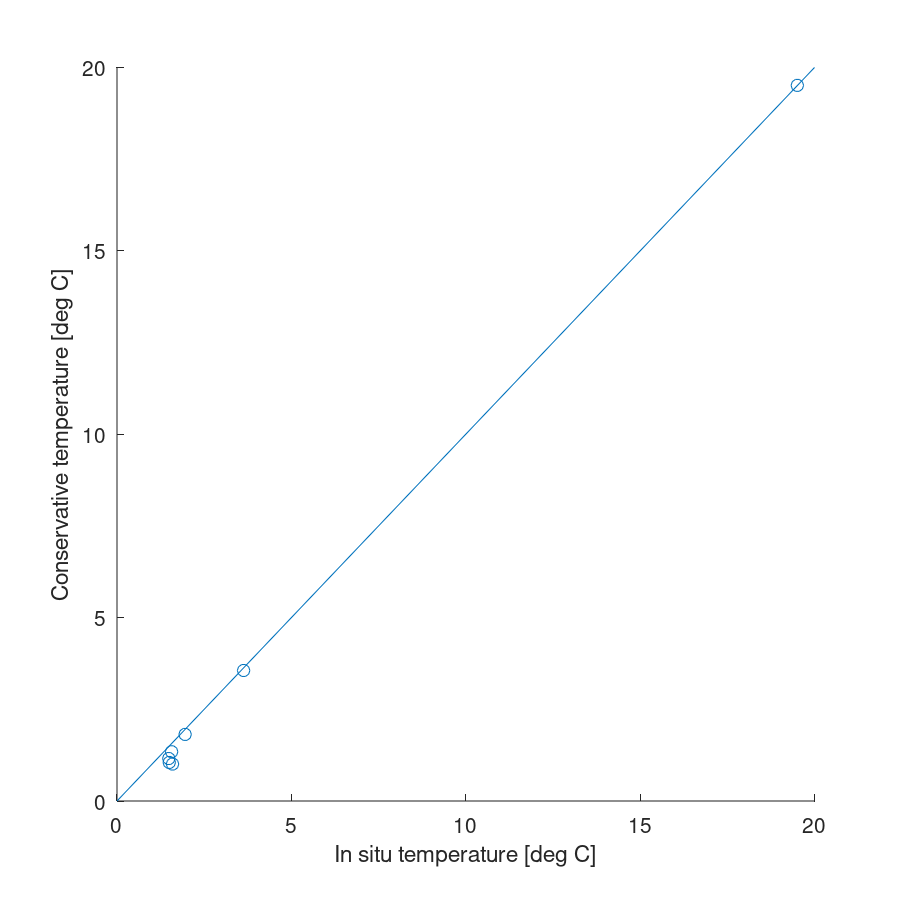
\includegraphics[scale=0.5]{t_vs_CT}
\par\end{centering}
\caption{}

\end{figure}

\begin{figure}
\begin{centering}
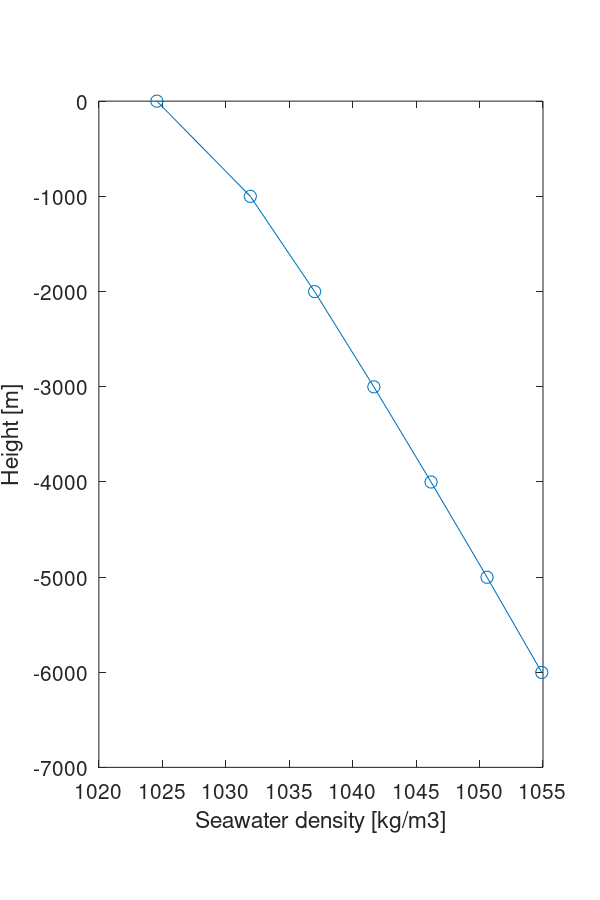
\includegraphics[scale=0.5]{density}
\par\end{centering}
\caption{}
\end{figure}

\begin{figure}
\begin{centering}
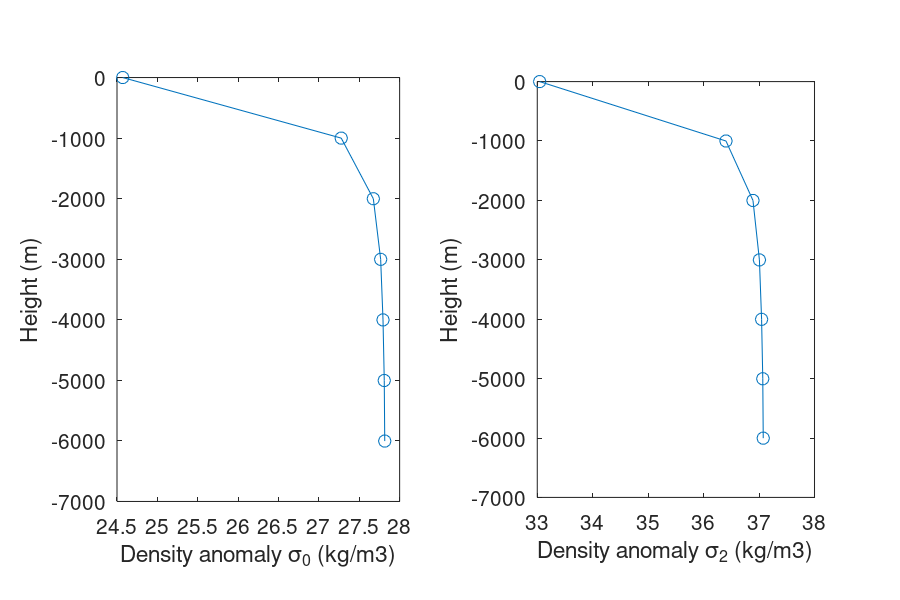
\includegraphics[scale=0.5]{sigma}
\par\end{centering}
\caption{}
\end{figure}
\begin{figure}
\begin{centering}
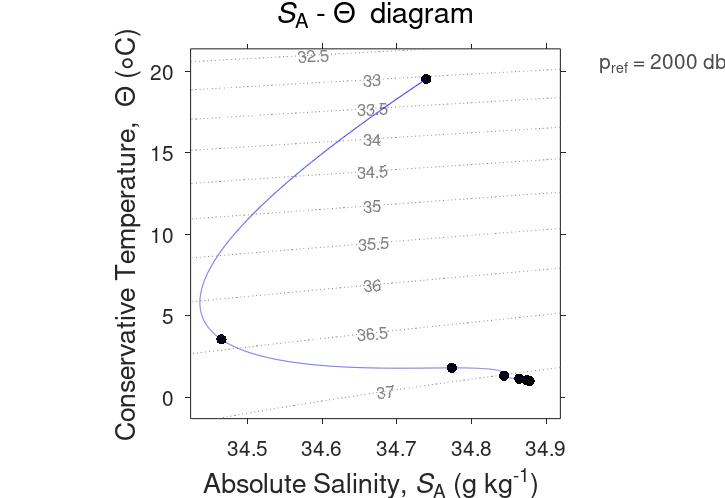
\includegraphics[scale=0.5]{SA-CT-ref2}
\par\end{centering}
\caption{}
\end{figure}

\begin{figure}
\begin{centering}
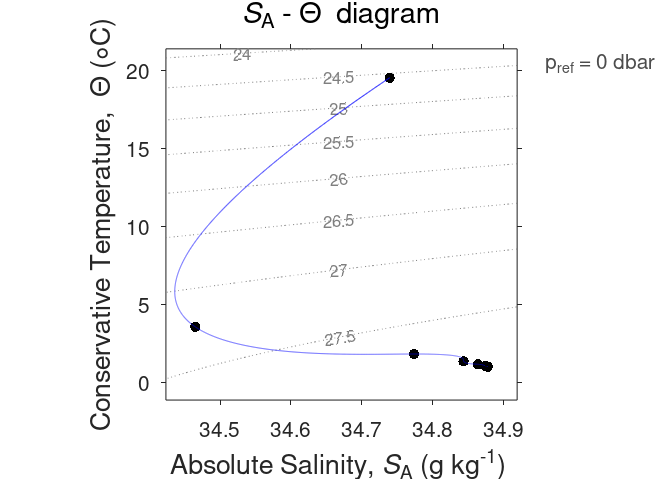
\includegraphics[scale=0.5]{SA-CT-ref0}
\par\end{centering}
\caption{}

\end{figure}


\section{Exercise: Processing real CTD data {[}60{]}}

In this exercise, you will use data from a processed CTD cast measured
during the winter 2016 campaign of the SA Agulhas II along the Good
Hope Line (from Cape Town to the Greenwich Meridian and then southward).
You will use the file \texttt{uctd03\_SOSX4\_2in2016.cnv} , which
contains the ``upcast'' data from the bottom to the surface. The
file has a header that explains the content and the variables measured
in each column (this will be explained by the tutor). \textbf{This
file is a text (ASCII) file. You will open it with the text editor
}(right click on the file and ``open with'')\textbf{ and you will
study the names of the variable for each column of the table (lines
starting with ``\# name''). }

\textbf{To import the data, the header must be removed, and a new
file only containing the values must be created}. Copy the file to
a new name and open it with the text editor. Delete all the lines
starting with {*} or \#.

Every figure you generate must have a title and the labels with the
proper units. The code must be commented in the Live Script, either
using a text cell or directly in the code cell.
\begin{enumerate}
\item {[}15{]} Import the data file using \texttt{importdata.} Create the
workspace variables that contain the following variables from the
data file: 
\begin{enumerate}
\item latitude and longitude in decimal degrees (note that in the file they
are in degrees and decimal minutes. You will need to convert them
after the import)
\item temperature, practical salinity, and pressure 
\end{enumerate}
\item {[}5{]} Plot the in situ temperature profile against height (set the
range of the Y axis between 0 and 1000 m depth using \texttt{ylim})
\item {[}10{]} Calculate (no plot) the profiles for:
\begin{enumerate}
\item Absolute salinity
\item Conservative temperature
\item $\sigma_{0}$ and $\sigma_{1}$
\end{enumerate}
\item {[}10{]} Plot the CT profile AND the freezing temperature profile
(against height, same range as above) on the same graph with different
colors. To compute the freezing temperature you will use the function
\texttt{gsw\_CT\_freezing\_poly}
\item {[}10{]} Plot a 2-panels' figure showing the vertical profiles of
$\sigma_{0}$ and $\sigma_{1}$. Also show the grid lines with the
\texttt{grid} command
\item {[}10{]} Plot the SA-CT diagrams for the 0 and 1000 dbar reference
pressures
\end{enumerate}
Submit your Live Script file, named \texttt{M2P2\_STUDENTNUMBER.mxl}.
\end{document}
